\section{JavaScript}
\label{javascript}

\textit{JavaScript} ist eine 1995 erschienene funktionale Skriptsprache mit dynamischem Typensystem, welche ursprünglich für die Erstellung von Websites mit dynamischen Inhalten erstellt wurde. Heutzutage ist JavaScript überall im Einsatz und hält den ersten Platz der meistverwendeten Programmiersprachen. \cite{technostacks2021}

\subsection{Kritik an JavaScript}

Obwohl JavaScript heutzutage eine der am weitesten verbreiteten Programmiersprachen ist und von vielen anerkannten Firmen aktiv verwendet wird, haben einige Entwickler dennoch Vorbehalte gegen die Nutzung von JavaScript.~\cite{keenetheng2016}

Die Begründung liegt in der oftmals eigenartigen Verhaltensweise der Sprache, welche man aus anderen Programmiersprachen nicht gewohnt ist. Listen wie \textit{wtfjs} von \textit{Denys Dovhan} zeigen Beispiele, wie komisch JavaScript wirklich sein kann. Einige Auszüge davon (siehe denysdovhan/wtfjs auf GitHub für alle Einträge):

\begin{code}[htp]
    \begin{center}
        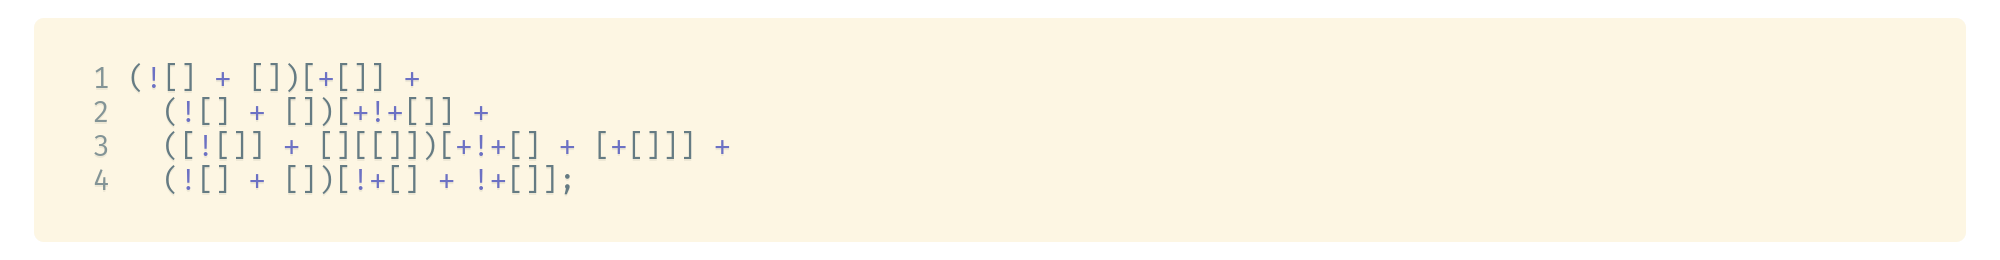
\includegraphics[width=1\textwidth]{images/JavaScript/fail.png}
        \vspace{-25pt}
        \caption{\glqq fail\grqq\space in JavaScript; diese Art von JavaScript ist auch bekannt als \textit{JSFuck}}
    \end{center}
\end{code}

\begin{code}[htp]
    \begin{center}
        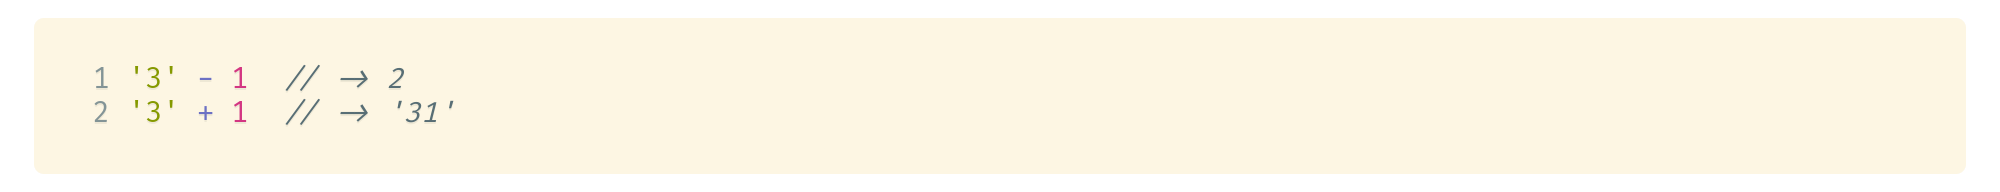
\includegraphics[width=1\textwidth]{images/JavaScript/coercing.png}
        \vspace{-25pt}
        \caption{Lustige Mathematik: Die Typenumwandlung (Coercing) in JavaScript ...}
    \end{center}
\end{code}